\documentclass[twocolumn]{article}[10pt]
\usepackage[english]{babel} 
\usepackage[latin1]{inputenc} 
\usepackage{times} 			% Default times font style
\usepackage[T1]{fontenc} 	% Font encoding
\usepackage{amsmath} 		% Math package
\usepackage{mathtools} 		% Adds the declare paired 
							% delimeter command to make costom \abs and \norm
\usepackage{breqn}		 	% Adds dmath environment for automated brakeline
\usepackage{xfrac}			% Adds slanted fractions (sfrac)
\usepackage{cancel}			% Adds the cancel command, a slash through the symbol(s)
\usepackage{tabularx}		% Adds adjustable width on tabulars
\usepackage{cuted}			% Adds the strip command, pagewidth text in a twocolumn
							% environment. 
\usepackage{hyperref}

% Start custom \abs \norm 
\DeclarePairedDelimiter\abs{\lvert}{\rvert}%
\DeclarePairedDelimiter\norm{\lVert}{\rVert}%
% Swap the definition of \abs* and \norm*, so that \abs
% and \norm resizes the size of the brackets, and the 
% starred version does not.
\makeatletter
\let\oldabs\abs
\def\abs{\@ifstar{\oldabs}{\oldabs*}}
%
\let\oldnorm\norm
\def\norm{\@ifstar{\oldnorm}{\oldnorm*}}
\makeatother
% End costum \abs \norm 

% TODO: Put comments on this section.
\newcommand{\eq}[1]{\begin{align*}#1\end{align*}}
\newcommand{\equ}[1]{\begin{align}#1\end{align}}
\renewcommand\vec[1]{{\bf #1}}
\newcommand{\OP}[1]{{\bf\widehat{#1}}}

\title{}

\begin{document}

\begin{titlepage}
\begin{center}

\textsc{\Large Variational Monte Carlo Simulations of
Atomic Systems}\\[0.5cm]
\rule{\linewidth}{0.5mm} \\[0.4cm]
{ \huge \bfseries  Part I}\\[0.10cm]
\rule{\linewidth}{0.5mm} \\[1.5cm]
\textsc{\Large FYS4411}\\
\textsc{\Large Computational Physics II}\\[1.5cm]
\textsc{}\\[1.5cm]

% Av hvem?
\begin{minipage}{0.49\textwidth}
    \begin{center} \large
		Daniel Marelius Bj\o rnstad
    \end{center}
\end{minipage}
\begin{minipage}{0.49\textwidth}
    \begin{center} \large
        Alexander Fleischer
    \end{center}
\end{minipage}

\vfill

% Dato nederst
\large{Dato: \today}

\end{center}
\end{titlepage}

\maketitle
%\newpage

\section{Introduction}
Github: \\ \url{https://github.com/lastis/FYS4411}

\section{Methods}
\subsection{Trial Wavefunction of Beryllium}

\eq{
   \psi_{T}({\bf r_1},{\bf r_2}, {\bf r_3}, {\bf r_4}) = 
   Det\left(\phi_{1}({\bf r_1}),\phi_{2}({\bf r_2}),
   \phi_{3}({\bf r_3}),\phi_{4}({\bf r_4})\right)
   \prod_{i<j}^{4}\exp{\left(\frac{r_{ij}}{2(1+\beta r_{ij})}\right)}, 
 }

\section{Results}
\subsection{Helium: Estimating $\alpha$ and $\beta$}
These parameters decide the minimal ground energy for the system, and both
should be adjusted simultaneously to reach the most optimal value of the
energy. First we sample the parameterspace of the first trial wave function. 
This function had a minimum of 1.66. This was the first value of $\alpha$ that was used in sampling the 
parameterspace with beta in the second trial wavefunction. 
This can  be seen in Figure \ref{fig:1} with mean error. 
Using the computed $\beta$-value we again
sampled the energy as a function of $\alpha$, which we concluded was 
the same as before. $\alpha$ is plotted in Figure \ref{fig:2}

\begin{figure}[h!]
	\centering
	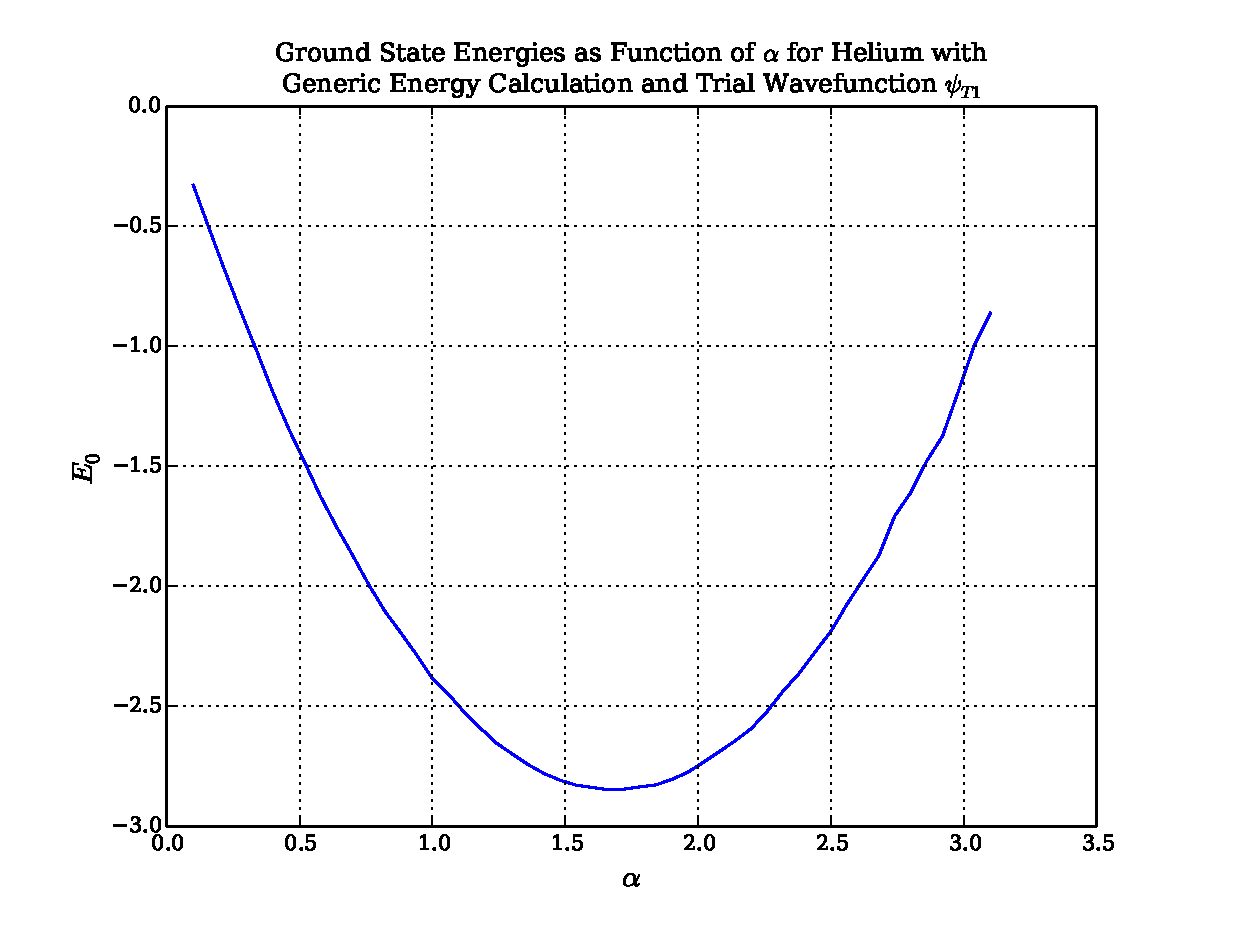
\includegraphics[width=80mm]{../res/heliumWave1Alpha/heliumWave1Alpha_alpha.eps}
	\caption{}\label{fig:2}
\end{figure}

\begin{figure}[h!]
	\centering
	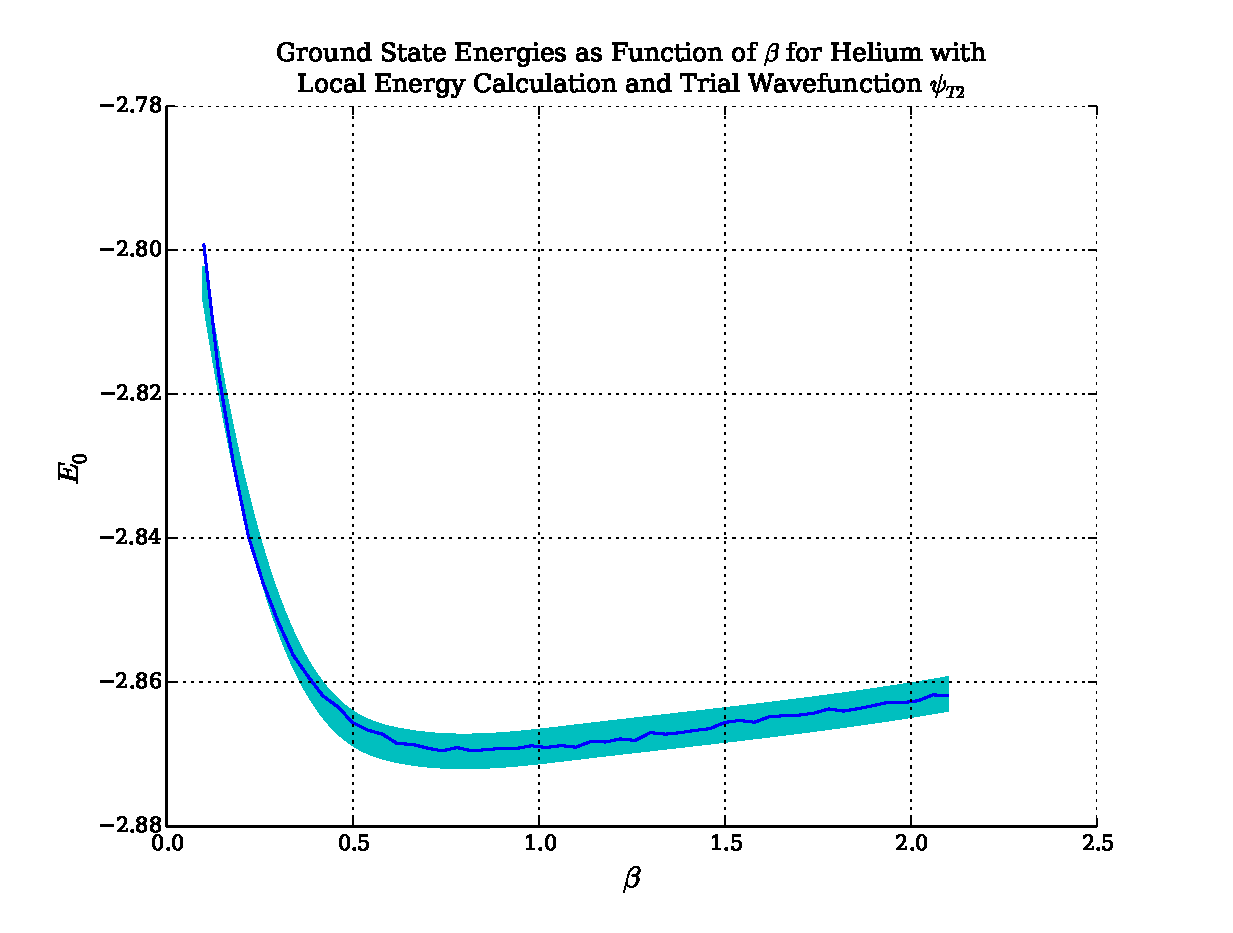
\includegraphics[width=80mm]{../res/heliumWave2Beta/heliumWave2Beta.eps}
	\caption{}\label{fig:1}
\end{figure}

\subsection{Helium: $\psi_{T1}$ and $\psi_{T2}$ }
Firstly we want to compare the first and second trial wavefunctions for Helium. 
The difference between these two are that there are no correlation term
in the first wavefunction. This makes computations much faster, but we
would expect that our results are farther away from the experimental 
value of the ground state. This is done using a numerical approximation 
of the local energy of the particles. The mean value of 
$\psi_{T1} = -2.84264$ and $\psi_{T2} = -2.87105$. The experimental value of
the ground state is about $-2.903$, thus we conclude that the second wavefunction is a better approximation.

\subsection{Helium: Closed Form Local Energy}
The local energy has a closed form solution for Helium, this has 
been implemented in Figure \ref{fig:3}. The closed-form solution should
give use a lower standard deviation than the numerical approximation
of the local energy because it is a closer approximation. 

\subsection{Helium: Importance Sampling}
Now we would like to see how the program does with importance sampling instead 
of static steplength. Importance sampling should also lower the standard 
deviation because it makes the walker sample the wavefunction in a
better way. The downside of importance sampling is that it takes about
twice as long time as the random walker. This is also shown in Figure \ref{fig:3}. 

\begin{figure}[h!]
	\centering
	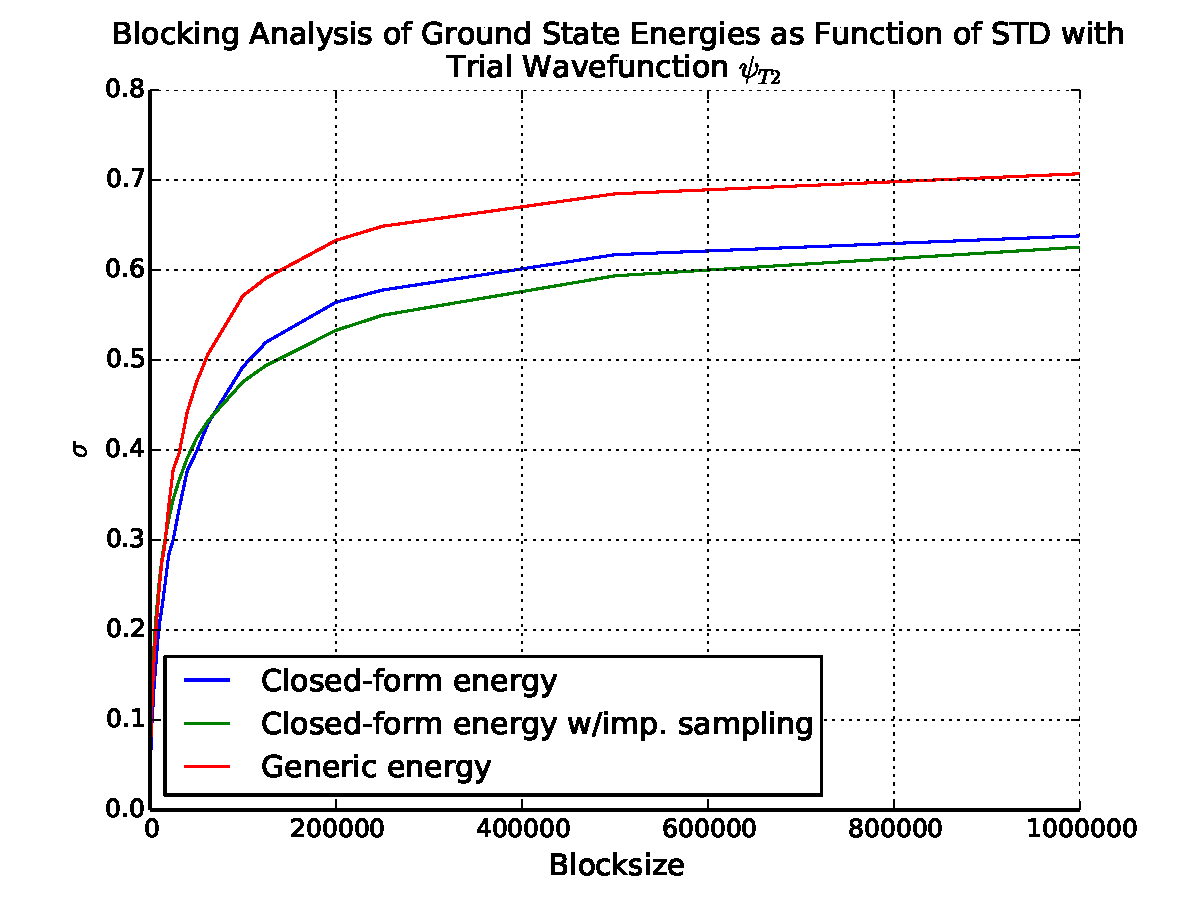
\includegraphics[width=80mm]{../res/heliumWave2ClosedImportanceGeneric/heliumWave2BlockingClosedImpGen.pdf}
	\caption{}\label{fig:3}
\end{figure}

\subsection{Helium: Evaluating Ground State and Density}
With our optimal parameters, we calculated the ground state and the density
function of Helium, Figure \ref{fig:4}. The standard deviation has been added as
a error bar along the curve.

Here we can see how the correlation factor effects the density. When
the Jastrow factor is added the electrons are repelled a bit farther 
away from the nucleus and the mean radius between the electrons increases
slightly. The mean distance increased from $1.316$ to $1.414$. 
\begin{figure}[h!]
	\centering
	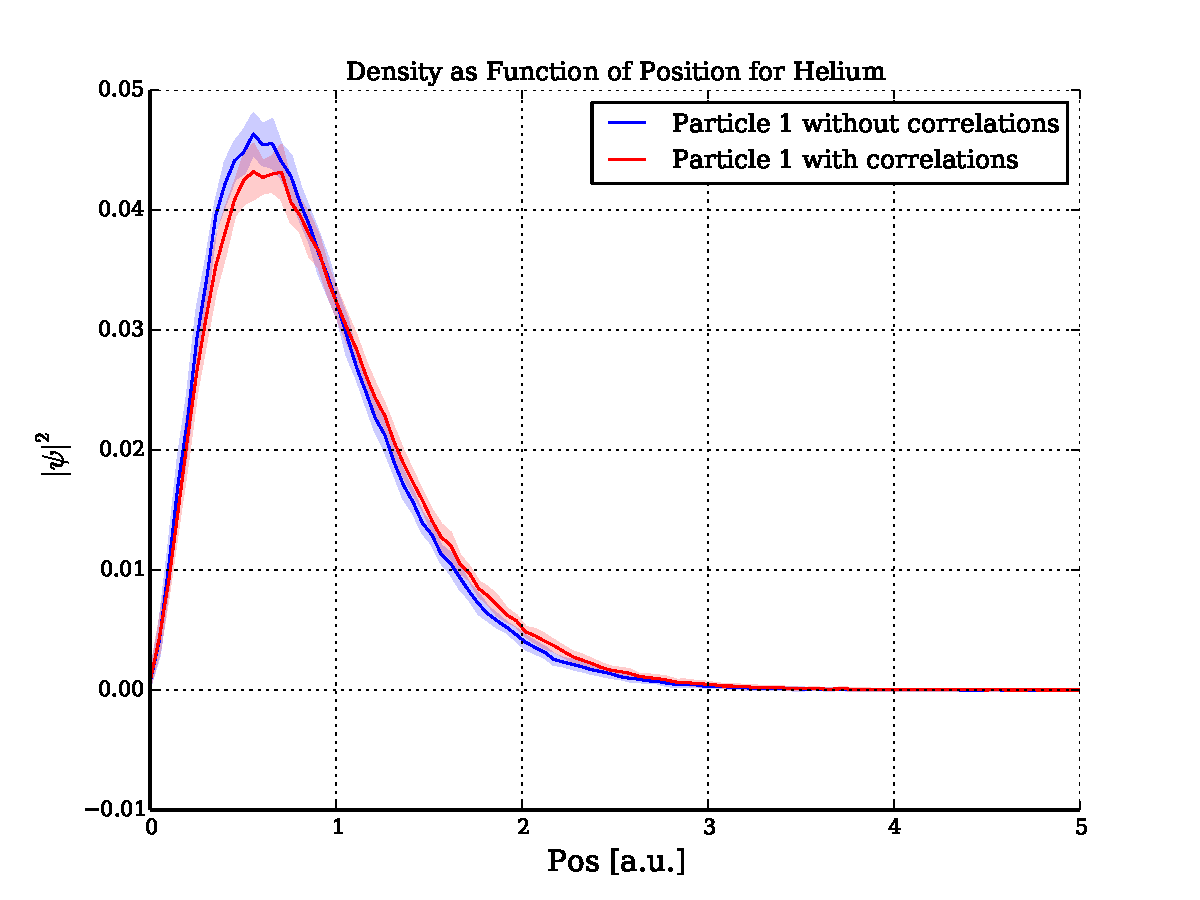
\includegraphics[width=80mm]{../res/heliumWave1Wave2Density/heliumWave1Wave2DensityPos1.pdf}
	\caption{}\label{fig:4}
\end{figure}

\subsection{Beryllium: Estimating $\alpha$ and $\beta$}
In Figure \ref{fig:5} a wide range of the parameter space has been sampled. As can be seen this area have an energy mean that are quite similar. Because of this
the parameters have been chosen to be $\alpha =  3.75$ and $\beta = 0.8$. 
\begin{figure}[h!]
	\centering
	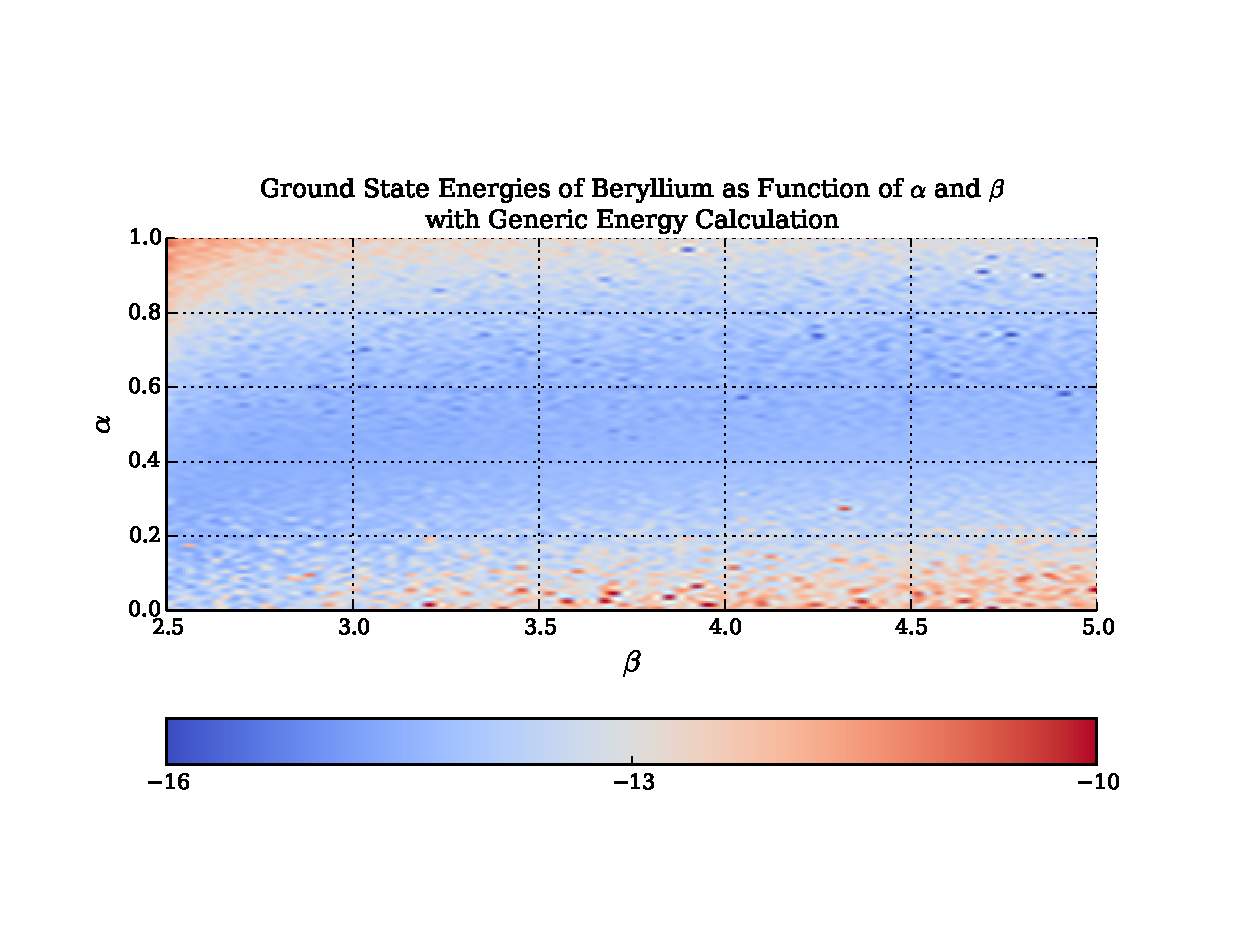
\includegraphics[width=80mm]{../res/berylliumAlphaBeta/berylliumAlphaBeta.eps}
	\caption{}\label{fig:5}
\end{figure}

\subsection{Beryllium: Comparing $\psi_{T1}$ and $\psi_{T2}$}
In Figure \ref{fig:6} we see the difference the Jastrow factor makes for Beryllium. 
We also notice the two clear peaks in the distribution. These are
the electron orbitals for 1s and 2s. Again this
correlation makes the electrons repel each other and pushes the distributions
farther apart. The mean distance increased from $1.669$ to $1.804$. 
The mean energy were $-19.9325$ and $-14.340$ respectively. A walue around
$-14$ is the experimental value of Beryllium and the value without the 
Jastrow factor is supposed to be $-20$. 
\begin{figure}[h!]
	\centering
	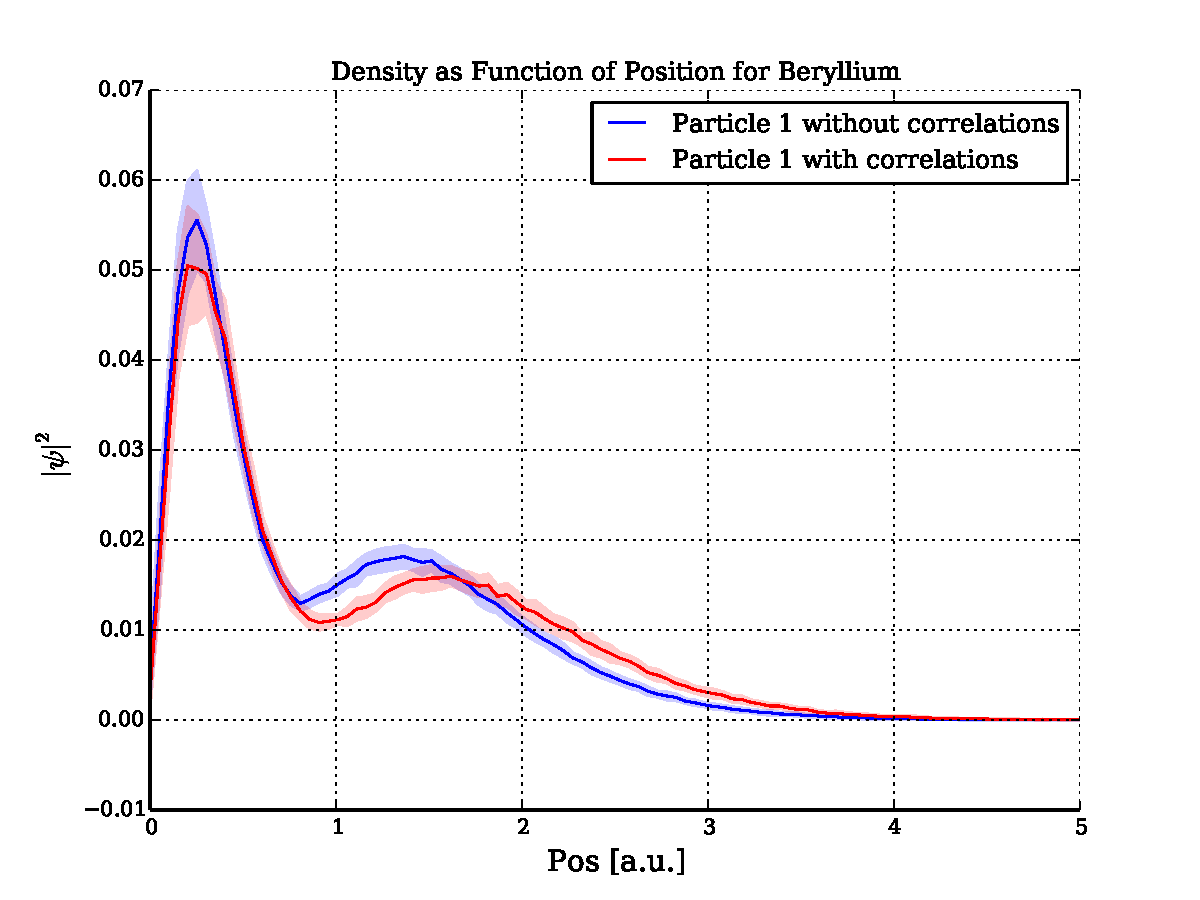
\includegraphics[width=80mm]{../res/berylliumWave1Wave2Density/berylliumWave1Wave2DensityPos1.pdf}
	\caption{}\label{fig:6}
\end{figure}




\section{Discussion}
\subsection{Parameter Space}
After estimating the parameters $\alpha$ and $\beta$ for 
Helium, we didn't adjust them in the late comparative trials. The reason
for this was that small changes in the parameters did not effect
our results considerably because the mean energies as well as the variance of the mean energies are similar. Our results was always close to 
$=-2.89$. The same conclusion was made for Beryllium, which
showed even harder to locate exact values of the paramters.  

The standard deviation of the mean was not considered when estimating the values 
of $\alpha$ and $\beta$. Performing blocking with our program would require full 
sampling of every step which stores about 10 mb for every value of $\alpha$ and $\beta$. 
\subsection{Testing of the Solver}
To varify that the solver works as intended, several unit tests
using UnitTest++ were created. The most important tests 
are those that estimate the one-body hamiltonian. this has
an analytical solution for both Helium and Beryllium, which is $-4$
and $-20$ respectively. 

The solutions for Hydrogen are also easy to calculate, and was estimated
to be $-0.5$ correctly.

\section{References}

\noindent Monte Carlo: Morten Hjorth-Jensen, Computational Physics, Lecture Notes Fall 2014, p. 345 (2014)\\

\noindent Importance Sampling: Morten Hjorth-Jensen, Computational Physics, Lecture Notes Fall 2014, p. 370 (2014)\\

\noindent Metropolis Algorithm: Morten Hjorth-Jensen, Computational Physics, Lecture Notes Fall 2014, p. 401 (2014)\\

\noindent Metropolis Algorithm: NICHOLAS
METROPOLIS,
ARIANNA
W.
ROSENBLUTH,
MARSHALL
N.
ROSENBLUTH,
AND
AUGUSTA
H.
TELLER,
Los
Alamos
Scientific
Laboratory,
Los
Alamos,
New
Mexico and EDWARD
TELLER,
*
Department
of
Physics,
University
of
Chicago, Chicago,
Illinois, The Journal of Chemical Physics \textbf{21}, p. 1087 (1953)\\

\noindent Blocking: H. Flyvbjerg and H. G. Petersen: Averages of correlated data, The Journal of Chemical Physics \textbf{91}, p. 461 (1989)
\end{document}
